\documentclass{article}
\usepackage{fullpage,amsmath,amssymb}
\usepackage{hyperref}
\usepackage[none]{hyphenat}
\usepackage{calc}  % arithmetic in length parameters
\usepackage{caption}
\usepackage{enumitem}  % more control over list formatting
\usepackage{fancyhdr}  % simpler headers and footers
\usepackage{geometry}  % page layout
\usepackage{lastpage}  % for last page number
\usepackage{listings}
\usepackage{parskip}
\usepackage{relsize}  % easier font size changes
\usepackage[normalem]{ulem}  % smarter underlining
\usepackage{url}  % verb-like typesetting of URLs
\usepackage{xcolor}
\usepackage{xfrac}  % nicer looking simple fractions for text and math

\definecolor{codegray}{rgb}{0.5,0.5,0.5}
\definecolor{codegreen}{rgb}{0,0.6,0}
\definecolor{codepurple}{rgb}{0.58,0,0.82}
\definecolor{backcolour}{rgb}{0.95,0.95,0.92}

\lstdefinestyle{mystyle}{
    backgroundcolor=\color{backcolour},   
    commentstyle=\color{codegreen},
    keywordstyle=\color{magenta},
    numberstyle=\tiny\color{codegray},
    stringstyle=\color{codepurple},
    basicstyle=\ttfamily\footnotesize,
    breakatwhitespace=false,         
    breaklines=true,                 
    captionpos=b,                    
    keepspaces=false,                 
    numbers=left,                    
    numbersep=5pt,                  
    showspaces=false,                
    showstringspaces=false,
    showtabs=false,                  
    tabsize=4
}
\lstset{style=mystyle}

\everymath{\displaystyle}

\newcommand{\arrayex}[1]{
    \begin{tabular}{|*{20}{c|}}
    \hline
    #1 \\
    \hline
    \end{tabular}
}

\setlength{\tabcolsep}{5pt}

\renewcommand{\arraystretch}{1}

%\usepackage[T1]{fontenc}  % use true 8-bit fonts
%\usepackage{slantsc}  % allow slanted small-caps
%\usepackage{microtype}  % perform various font optimizations
%% Use Palatino-based monospace instead of kpfonts' default.
%\usepackage{newpxtext}

% Common macros.
%%  Common macros for the course CSC263H1 at the University of Toronto.
%%
%%  Copyright (c) 2014 Francois Pitt <fpitt@cs.utoronto.ca>
%%  last updated at 17:53 (EDT) on Sun 19 Oct 2014
%%
%%  CC BY-SA 4.0
%%  This work (the current file named 'macros-263.tex') is licensed under
%%  the Creative Commons Attribution-ShareAlike 4.0 International License.
%%  To view a copy of this license, visit
%%      http://creativecommons.org/licenses/by-sa/4.0/
%%  or send a letter to: Creative Commons, 444 Castro Street, Suite 900,
%%  Mountain View, California, 94041, USA.
%%  This is a human-readable summary of (and not a substitute for) the
%%  license.
%%  You are free to:
%%      Share -- copy and redistribute the material in any medium or format
%%      Adapt -- remix, transform, and build upon the material for any
%%          purpose, even commercially.
%%      The licensor cannot revoke these freedoms as long as you follow the
%%          license terms.
%%  Under the following terms:
%%      Attribution -- You must give appropriate credit, provide a link to
%%          the license, and indicate if changes were made. You may do so in
%%          any reasonable manner, but not in any way that suggests the
%%          licensor endorses you or your use.
%%      ShareAlike -- If you remix, transform, or build upon the material,
%%          you must distribute your contributions under the same license as
%%          the original.
%%      No additional restrictions -- You may not apply legal terms or
%%          technological measures that legally restrict others from doing
%%          anything the license permits.
%%  Notices:
%%      You do not have to comply with the license for elements of the
%%      material in the public domain or where your use is permitted by an
%%      applicable exception or limitation.
%%      No warranties are given. The license may not give you all of the
%%      permissions necessary for your intended use. For example, other
%%      rights such as publicity, privacy, or moral rights may limit how you
%%      use the material.

% Redefine \today in the style "DD Month YYYY".
\renewcommand*\today
 {\number\day\space\ifcase\month\or January\or February\or March\or
  April\or May\or June\or July\or August\or September\or October\or
  November\or December\fi\space\number\year}

% TeX trick so that math symbols are bold when text is.
\let\seiresfb\bfseries\def\bfseries{\boldmath\seiresfb}
\let\seiresdm\mdseries\def\mdseries{\unboldmath\seiresdm}

% Centered version of \llap and \rlap.
\providecommand*\clap[1]{\hbox to 0pt{\hss#1\hss}}

% Spacing macros with default argument.
\providecommand*\vfillstretch[1][1]{\vspace*{\stretch{#1}}}
\providecommand*\hfillstretch[1][1]{\hspace*{\stretch{#1}}}

% Abbreviations of latin phrases.
\let\latinabb\empty  % no special formatting
\providecommand*\ie{\latinabb{i.e.}}
\providecommand*\eg{\latinabb{e.g.}}
\providecommand*\etc{\latinabb{etc}}
\providecommand*\vs{\latinabb{vs}}

% General fonts and characters.
\let\longemph\textsl  % alternate way to emphasize
\let\strong\textbf  % strong emphasis
\let\code\texttt  % code fragments
\let\var\textsl  % multi-letter variables
\let\pred\mathbf  % predicates
\providecommand*\stup{\textsuperscript{st}}
\providecommand*\ndup{\textsuperscript{nd}}
\providecommand*\rdup{\textsuperscript{rd}}
\providecommand*\thup{\textsuperscript{th}}
\newcommand*\bbmath[1]{\ensuremath{\mathbb{#1}}}  % requires amssymb
\providecommand*\N{\bbmath{N}}  % requires amssymb
\providecommand*\Z{\bbmath{Z}}  % requires amssymb
\providecommand*\Q{\bbmath{Q}}  % requires amssymb
\providecommand*\R{\bbmath{R}}  % requires amssymb
\providecommand*\bigOh{\mathcal{O}}
\providecommand*\onehalf{\ensuremath{{}^1\!\!/\!_2}}
\providecommand*\letlinebreak{\penalty\exhyphenpenalty}
\providecommand*\halfthinspace{\kern.083333em}
\providecommand*\dash
   {\letlinebreak\halfthinspace---\halfthinspace\letlinebreak}
\let\per\slash  % for convenience

% For defined terms -- requires package ulem.
\newcommand*\defn[1]{\uline{\textit{#1}}}
%\setlength{\ULdepth}{.2ex}

% General math macros.
\newcommand*\hiderel[1]{\mathrel{\hphantom{#1}}}
\providecommand*\comp[1]{\overline{#1}}  % set complement
\providecommand*\emptystr{\varepsilon}  % empty string
\providecommand*\lxor{\mathbin\oplus}  % exclusive or
\providecommand*\cat{\cdot}  % string concatenation
% Floors and ceilings, with optional size-changing command, e.g.,
% \floor[\Big]{x/2} becomes '\Big\lfloor{x/2}\Big\rfloor'.
\providecommand*\floor[2][]{{#1\lfloor}{#2}{#1\rfloor}}
\providecommand*\ceil[2][]{{#1\lceil}{#2}{#1\rceil}}
\providecommand*\lcm{\operatorname{lcm}}  % requires amsmath
\providecommand*\size{\operatorname{size}}  % requires amsmath
\providecommand*\len{\operatorname{len}}  % requires amsmath
\providecommand*\divides{\mathrel{|}}

% Redefined symbols from amssymb.
\renewcommand*\emptyset{\varnothing}  % rounder than default
\let\bigiff\iff
\renewcommand*\iff{\mathrel{\Leftrightarrow}}  % smaller than default
\let\bigimplies\implies
\renewcommand*\implies{\mathrel{\Rightarrow}}  % smaller than default
\renewcommand*\ge{\geqslant}  % with slanted line under the > sign
\renewcommand*\le{\leqslant}  % with slanted line under the < sign

% For algorithms, using either CLRS-style or Python-style pseudocode.
\let\ADT\textsc  % ADT names
\let\proc\textsc  % function names
\let\const\textsc  % constants (True, False, etc.)
\let\kw\textbf  % keywords (if, while, etc.)
\providecommand*\comm[1]{\textsl{\#\space#1}}  % comments
\providecommand*\opgets[1]{\mathrel{#1=}}
\providecommand*\eq{\mathrel{==}}
\providecommand*\True{\const{True}}
\providecommand*\False{\const{False}}
\providecommand*\None{\const{None}}
\providecommand*\cmod{\mathbin{\%}}
\providecommand*\nil{\const{nil}}

% Checkboxes and checklists.
% \checkmark already defined in amssymb
\makeatletter
\@ifpackageloaded{kpfonts}
   {\newcommand*\exmark{$\times$}}
   {\newcommand*\exmark{{\boldmath$\times$}}}
\makeatother
\newlength\exmarksize
\newlength\exmarkdepth
\newcommand*\checkbox[1][]
   {\settoheight\exmarksize{\exmark}
    \settodepth\exmarkdepth{\exmark}
    \addtolength\exmarksize{-\exmarkdepth}
    {\setlength\fboxrule{.1ex}\setlength\fboxsep{.1ex}%
    \fbox{\rule{0pt}{\exmarksize}\makebox[\exmarksize]{\smash{#1}}}}}
\newcommand*\checkedbox{\checkbox[\raisebox{.1ex}{\kern.2em$\checkmark$}]}
\newcommand*\exedbox{\checkbox[\exmark]}
\newenvironment*{checklist}{\begin{list}{\checkbox}{}}{\end{list}}
\newcommand*\checkeditem{\item[\checkedbox]}
\newcommand*\exeditem{\item[\exedbox]}
\newcommand*\boxeditem[1][]{\item[{\checkbox[#1]}]}

% Macros for drawing "underline" rules and half-boxes.
\providecommand*\urule[2][.5pt]{\rule[-.4ex]{#2}{#1}} % "underline" rule
% Underlined text box (with optional positioning argument).
\providecommand*\ubox[3][c]{\rlap{\urule{#2}}\makebox[#2][#1]{#3}}
% Underlined text box with caption (and optional caption positioning).
\providecommand*\capbox[5][c]{\ifx\empty#2\empty
    \else\rlap{\raisebox{-\baselineskip}{\makebox[#3][#1]{#2}}}\fi
    \ubox[#4]{#3}{#5}}

% For student numbers.
\providecommand*\hb{\urule{1.2em}}      % horizontal bar
\providecommand*\vb{\urule[1ex]{.5pt}}  % vertical bar
\providecommand*\studentnumberboxes     % now 10-digits long!
   {\vb\hb\vb\hb\vb\hb\vb\hb\vb\hb\vb\hb\vb\hb\vb\hb\vb\hb\vb\hb\vb}
\newlength\numberboxwidth
\settowidth\numberboxwidth{\studentnumberboxes}

% Command to format sample solutions for tutorials.
\newcommand\samplesolution[1]
   {\ifsolutions\begin{quote}\sffamily{#1}\end{quote}\fi}

% Marking-related macros.
\providecommand*\markitem[2][]
   {\item{\bfseries#2}\ifx\empty#1\empty\else
    \space[$#1$ mark\ifnum#1>1 s\fi]\fi:\quad\ignorespaces}
\providecommand*\errorcode[2][]
   {\item{\bfseries error code #2}\ifx\empty#1\empty\else
    \space[#1]\fi:\quad\ignorespaces}
\providecommand*\commonerror[1][]
   {\item{\bfseries common error}\ifx\empty#1\empty\else
    \space[#1]\fi:\quad\ignorespaces}
\makeatletter
\providecommand*\heading[1]%
   {\@startsection{heading}{9}{0pt}{-.75ex plus -1.5ex minus -.5ex}
    {-.5em plus -.5em minus -.25em}{\normalfont}*{\textsc{#1}}\mbox{}}
\makeatother



\geometry{a4paper, margin=1in, headheight=15pt, headsep=20pt}

\pagestyle{fancy}
\fancyhf{}
\fancyhead[L]{CSC311 Summer 2024}
\fancyhead[R]{Final Project}
\fancyfoot[C]{\thepage}


\title{Part B}
\date{\vspace{-10.0ex}}
\hypersetup{pdfpagemode=Fullscreen,
    colorlinks=true,
    linkfileprefix={}}


\begin{document}
\maketitle
\thispagestyle{fancy}

\section*{Formal Description}

The performance of the IRT algorithm in part A is not satisfactory. We believe that the main reason is that a single decision tree is a high-variance model. We believe that the decision tree in part A overfits the training data, which makes the model's generalization ability poor.

Therefore, we decided to reduce the variance by averaging the predictions of multiple decision trees using a random forest. Each tree is trained on a different random subset of the training data. The results are aggregated at the end to make the model more robust by smoothing the data.

\section*{Algorithm Box}

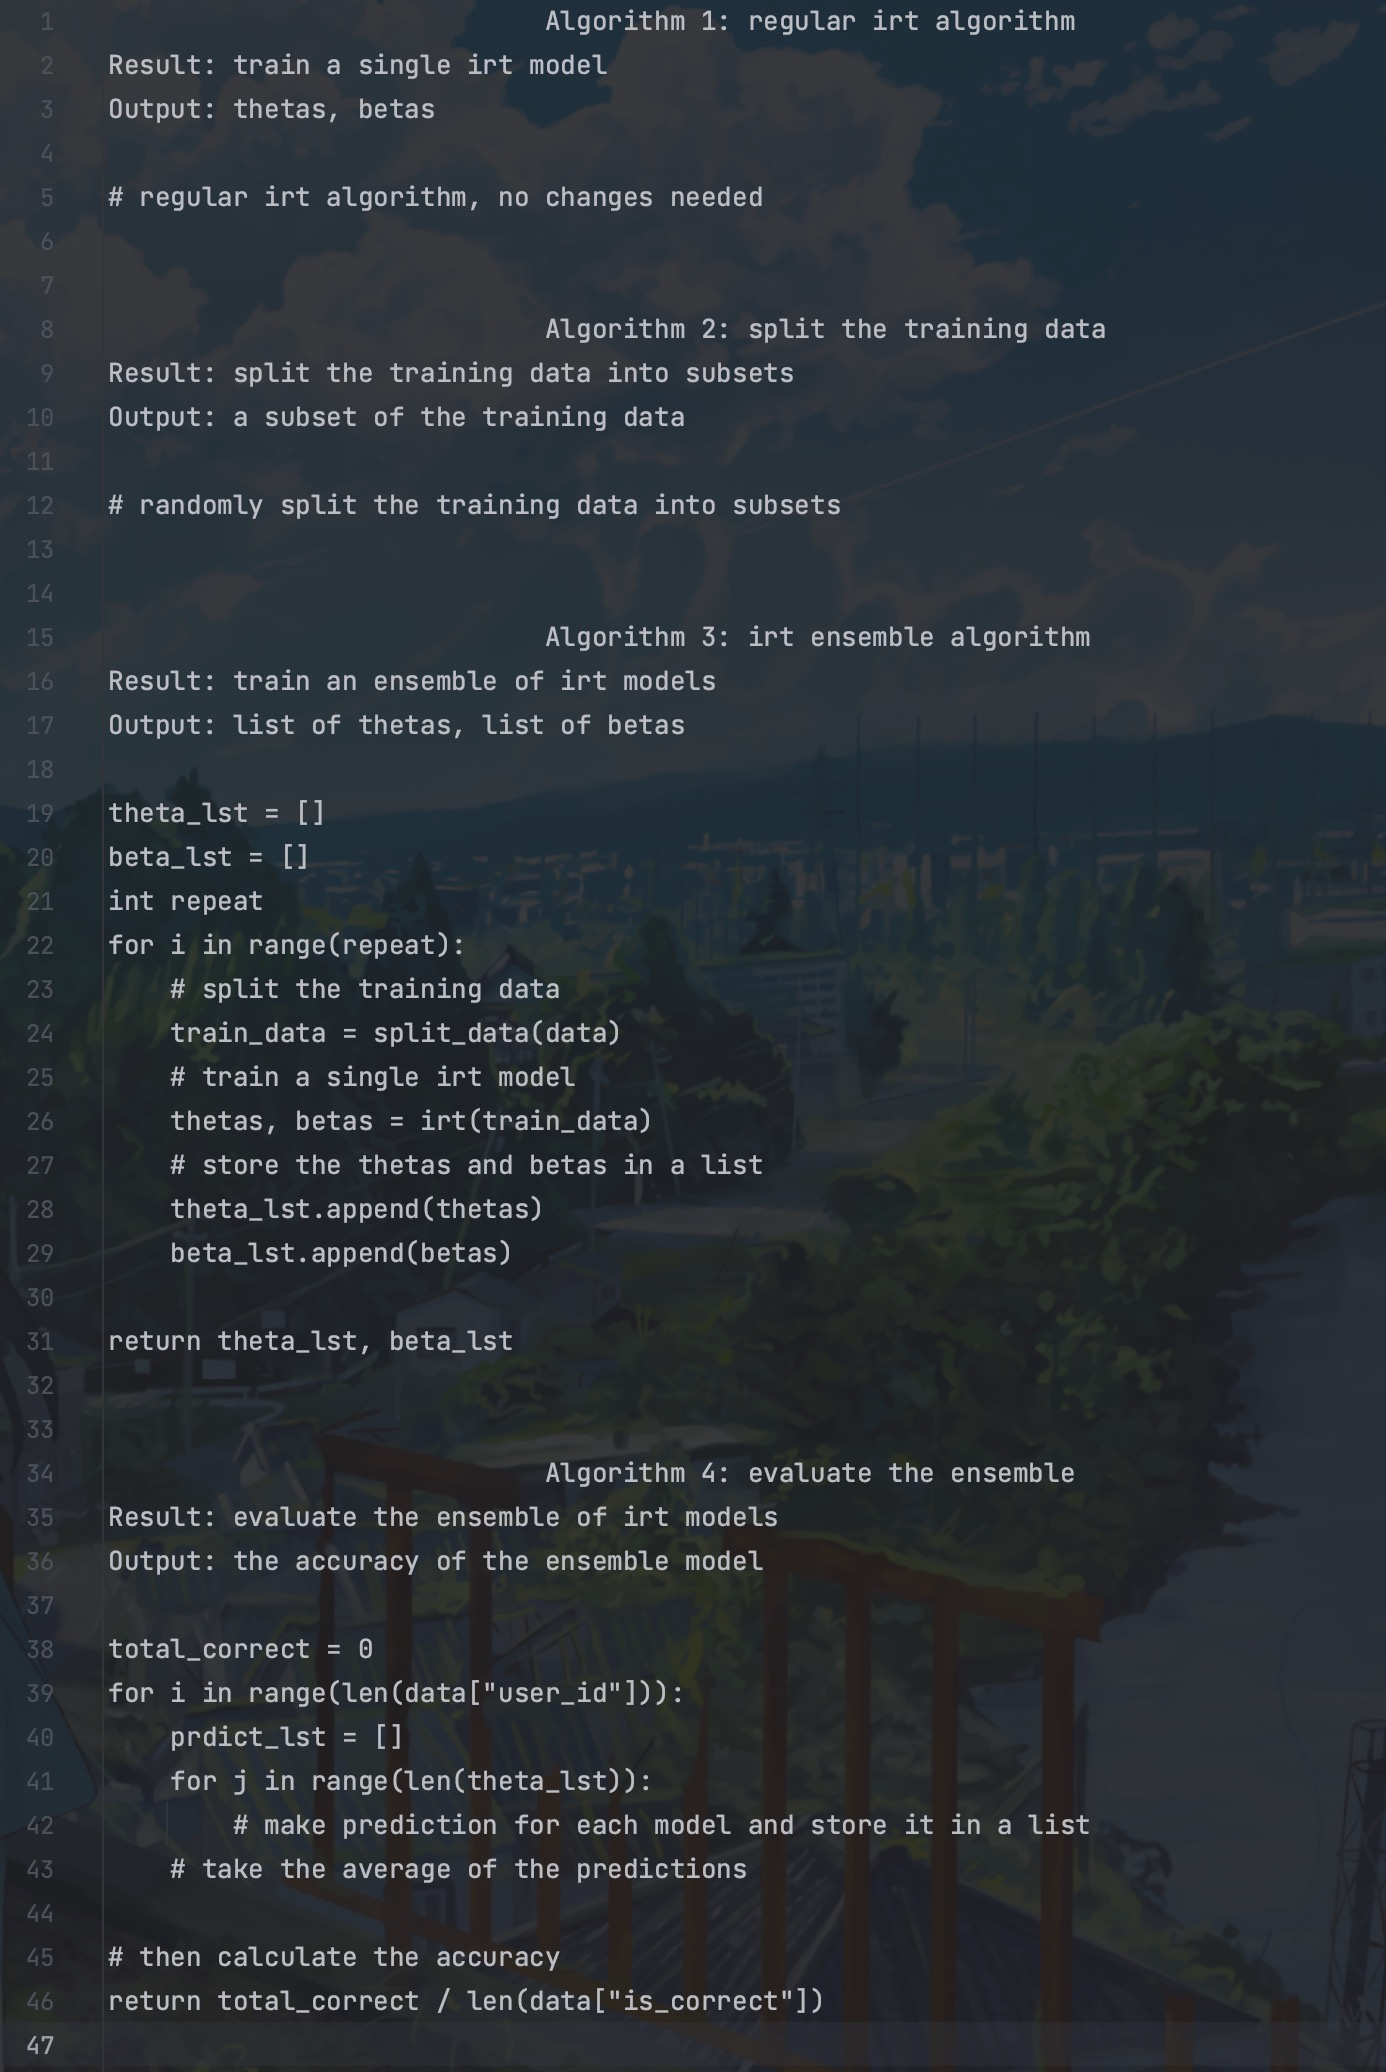
\includegraphics[width=0.7\linewidth]{6051723192250_.pic.jpg}

By training multiple decision trees on different data subsets in the form of random forests, the overfitting problem of the model can be reduced.

\section*{Idea Diagram}

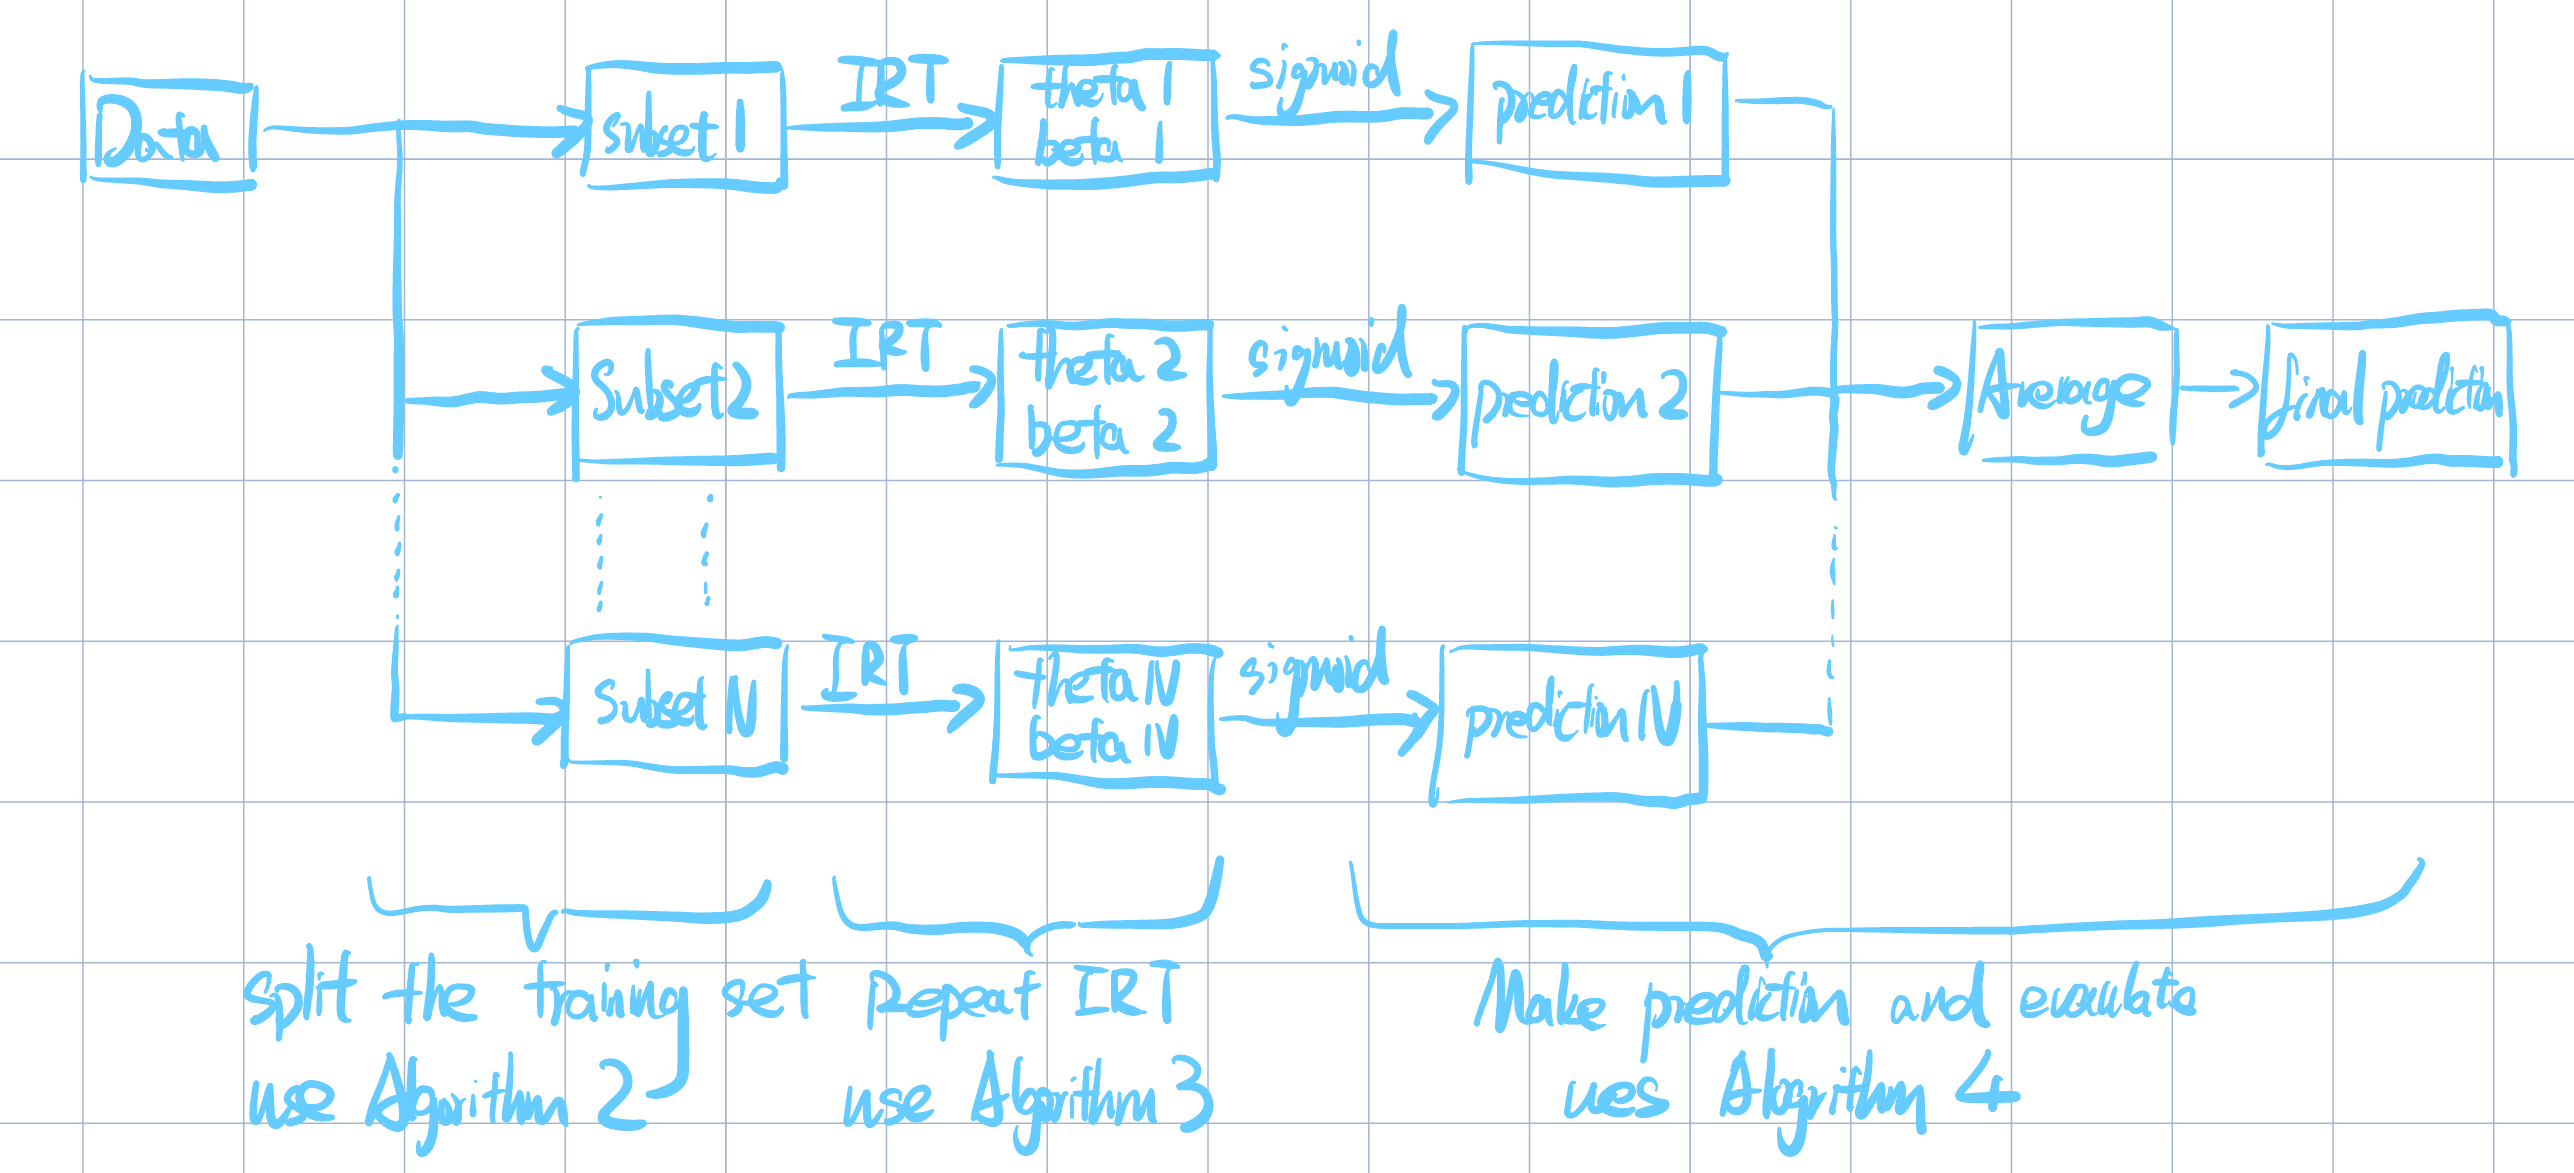
\includegraphics[width=1.0\linewidth]{笔记 2024年8月9日.jpeg}

\section*{Comparison or Demonstration}

For comparison, when using the single irt algorithm, we obtained the following statistics. We use this group of data as the baseline models:

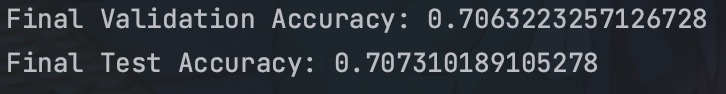
\includegraphics[width=0.7\linewidth]{6061723195551_.pic.jpg}

When using a random forest consisting of two decision trees, we get the following statistics:

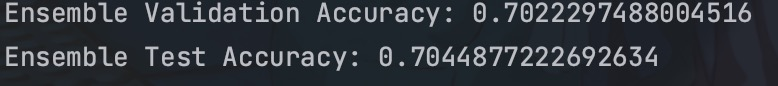
\includegraphics[width=0.7\linewidth]{6081723195750_.pic.jpg}

When using a random forest consisting of three decision trees, we get the following statistics:

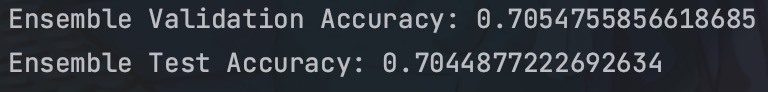
\includegraphics[width=0.7\linewidth]{6101723195879_.pic.jpg}

When using a random forest consisting of four decision trees, we get the following statistics:

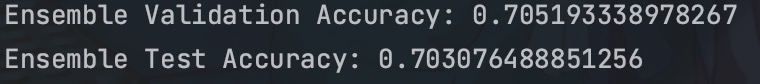
\includegraphics[width=0.7\linewidth]{6121723196137_.pic.jpg}
    
After comparison, our model does not significantly improve the accuracy.

\section*{Experiment to Test Our Hypothesis}

We use the accuracy of the training dataset and the accuracy of the validation dataset to determine whether the model has signs of overfitting. If the training accuracy is significantly higher than the validation accuracy, it means that the model is too sensitive to the training dataset and has signs of overfitting. On the contrary, if the training accuracy and validation accuracy are close, it means that the model does not have overfitting.

The test accuracy of the original model is as follows:

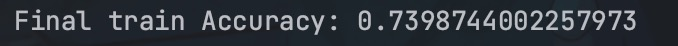
\includegraphics[width=0.7\linewidth]{6071723195572_.pic.jpg}

We can see that the training accuracy of the original model is significantly higher than the validation accuracy, indicating that the original model may be overfitting.

The random forests consisting of 2, 3, and 4 decision trees have the following statistics:

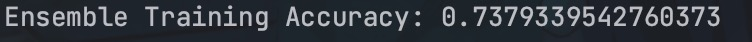
\includegraphics[width=0.7\linewidth]{6091723195756_.pic.jpg}

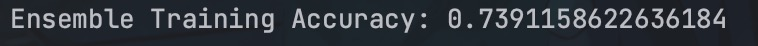
\includegraphics[width=0.7\linewidth]{6111723195885_.pic.jpg}

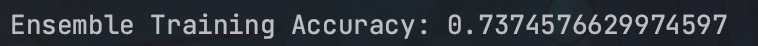
\includegraphics[width=0.7\linewidth]{6131723196143_.pic.jpg}

Unfortunately, Random Forest only slightly reduces the gap between training accuracy and validation accuracy, and the overfitting problem still exists.

\section*{Limitations}

As mentioned above, implementing Random Forest algorithm did not improve our original model significantly. This could be due to the following reasons:
\begin{itemize}
    \item The given dataset is not large enough or diverse enough. Random Forest is known to perform well on large-scale datasets with many features. In our improved model, we split the dataset into many subsets and trained a Random Forest model on each subset. However, the dataset may not be large enough to benefit from this approach.
    
    Hence, changing the dataset may improve the performance of the Random Forest algorithm.
    
    \item In our Random Forest algorithm, we assumes all predictions from the base models are equally important and we average all predictions of each decision tree to get the final prediction. This may not be the case in practice. Some models may perform better on certain types of data, and simply averaging their predictions may not be the best approach.
    
    We can use a weighted average of the predictions to give more importance to the better performing models, but this requires tuning the weights, which can be time-consuming.

    \item When ensembling multiple models, we need to ensure generalization. It may be because the base models are too similar and the overfitting problem still exists.
    
    We may need to use regularization to limit the complexity of the base models.
   
    \item The Random Forest algorithm is computationally expensive. It requires a lot of time to tune the hyperparameters and train the model. We may not have been able to find the best hyperparameters in the time we had.
   
    \item IRT model itself may be limited in predicting the student's performance. If we integrate more complex models in the ensemble, we may improve the performance of the model.
\end{itemize}

\section*{Contributions}

\subsection*{Part A}

\begin{itemize}
    \item Quesion 1 and 2: Mingzhe Zhang
    
    \item Question 3 and 4: Zhiyuan Meng
\end{itemize}

\subsection*{Part B}

\begin{itemize}
    \item Question 1, 2 and 3: Zhiyuan Meng
    
    \item Question 4: Mingzhe Zhang
\end{itemize}

\end{document}
